\chapter{Projekt}
\section{Interfejs użytkownika}

\begin{figure}[H]
\caption{Tryb widoku grafu}
\centering
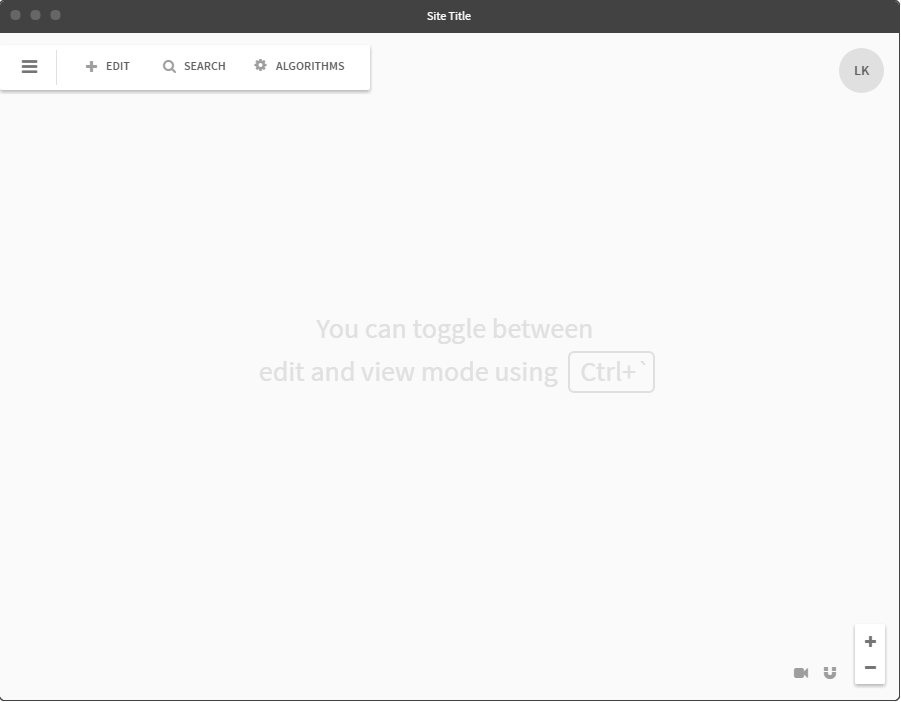
\includegraphics[width=\textwidth]{mock-view.png}
\end{figure}

\begin{figure}[H]
\caption{Tryb edycji grafu}
\centering
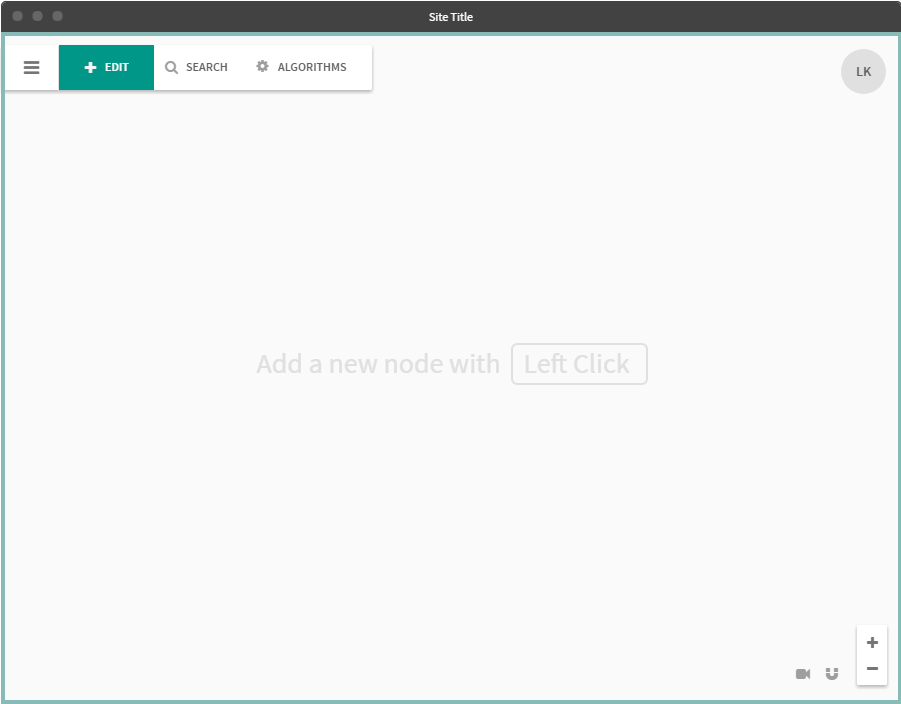
\includegraphics[width=\textwidth]{mock-edit.png}
\end{figure}

\begin{figure}[H]
\caption{Widok menu}
\centering
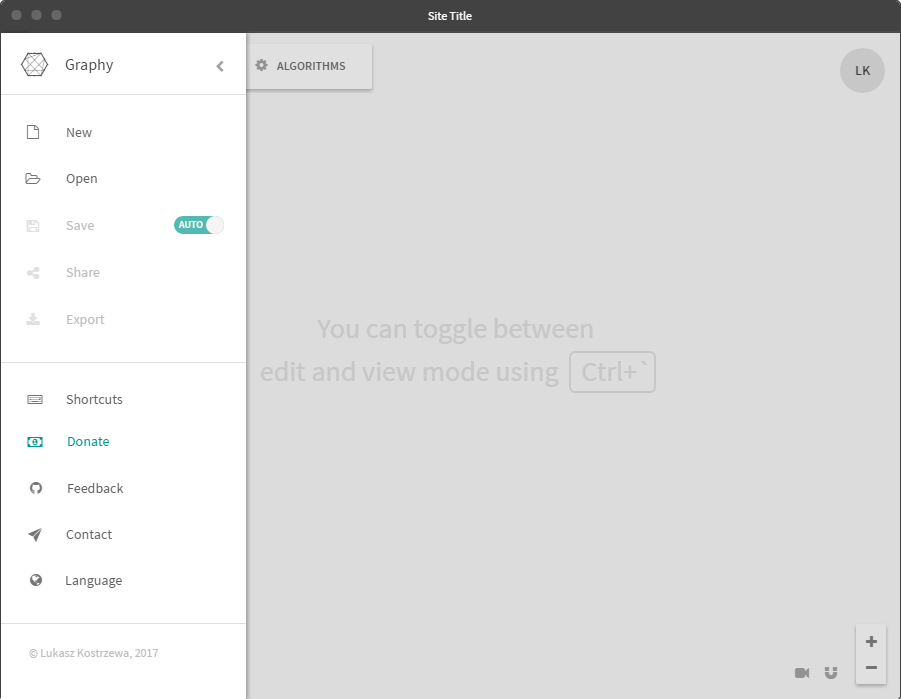
\includegraphics[width=\textwidth]{mock-menu.png}
\end{figure}

\begin{figure}[H]
\caption{Menu kontekstowe i informacja o ostatniej akcji}
\centering
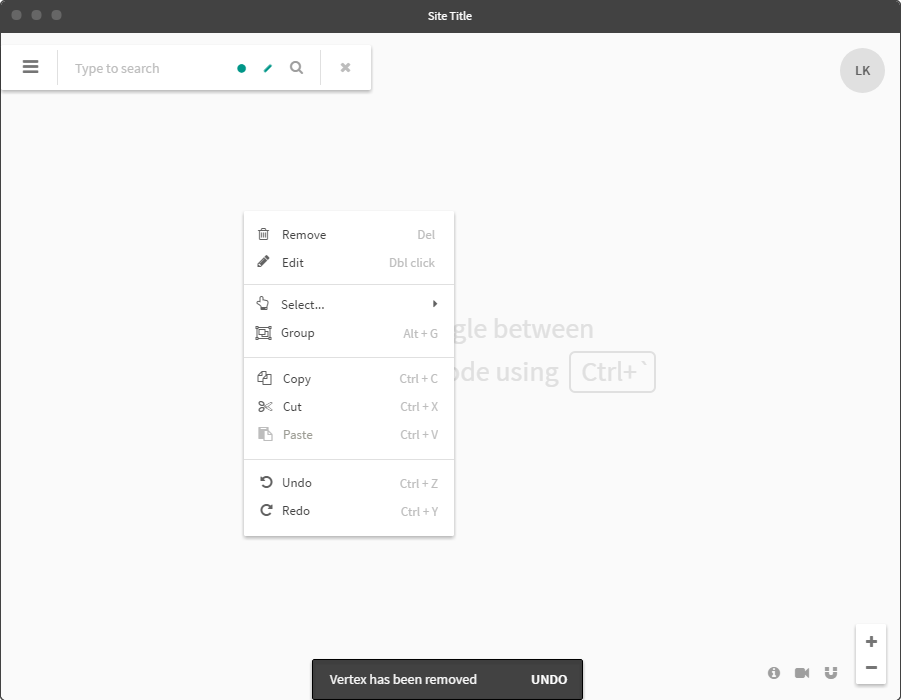
\includegraphics[width=\textwidth]{mock-context-menu.png}
\end{figure}